\lstinputlisting[language=bash,basicstyle=\small]{python_codes/fieldstone_72/keywords.ascii}

\begin{center}
Code at \url{https://github.com/cedrict/fieldstone/tree/master/python_codes/fieldstone_72}
\end{center}

\par\noindent\rule{\textwidth}{0.4pt}

%%%%%%%%%%%%%%%%%%%%%%%%%%%%%%%%%%%%%%%%%%%%%%%%%%%%%%%%%%%%%%%%%%%%%%%%%%%%%%%%%%%%%%%%%%%%%%%%%%%%

\index{stopics}{$Q_1^+\times Q_1$}


%--------------------------------------
\section*{Manufactured solution \#1}

The analytical solution originates in \textcite{lami17} (2017).
The velocity and pressure are given by
\begin{eqnarray}
u(x,y)&=&-2x^2y(2y-1)(x-1)^2(y-1) \\
v(x,y)&=& 2xy^2(2x-1)(x-1)(y-1)^2 \\
p(x,y)&=& x(1-x)(1-2y)
\end{eqnarray}
Boundary conditions are no-slip on all sides of the unit square. 
The corresponding body force terms are derived in Section~\ref{MMM-ss:mms11}. 


The quadrilateral MINI element used here also originates in the same article 
and comes in two flavours with two different bubble functions $b_1$ and $b_2$
as explained in Section~\ref{MMM-ss:quadmini}.
The two bubble functions are (in reduced coordinates $-1 \leq r,s \leq 1$):
\begin{eqnarray}
b_1(r,s) &=& (1-r^2)(1-s^2)\cdot (1-r)(1-s)\\
b_2(r,s) &=& (1-r^2)(1-s^2)\cdot (1+\beta(r+s))
\end{eqnarray}
The common term to both bubbles insures that the bubble is exactly zero on all four edges of the 
element. What differentiates them is the remaining term, which is bilinear ($b_1$) or linear ($b_2$). 
Both also satisfy $b_1(0,0)=b_2(0,0)=1$. The paper uses $\beta=1/4$.

The velocity and pressure fields for the benchmark are shown hereunder:
\begin{center}
\includegraphics[width=7cm]{python_codes/fieldstone_72/results/mms/vel}
\includegraphics[width=7cm]{python_codes/fieldstone_72/results/mms/p}
\end{center}

During the debugging process I ended up 
implementing various Gauss quadratures schemes, from $2^2$ to $6^2$ points but the results
show that $2^2$ quadrature points per element are sufficient since the more expensive quadratures
yield identical results. 
The results from the article are somewhat different than mine but I suspect that what the 
author measured could be different than what I measure (see Table 1,2 in \cite{lami17}). 
The trends are similar though, with $b_2$ performing better than $b_1$:

\begin{center}
\includegraphics[width=8cm]{python_codes/fieldstone_72/results/mms/errors_v}
\includegraphics[width=8cm]{python_codes/fieldstone_72/results/mms/errors_p}\\
{\captionfont Left: velocity error in $L_2$ norm; Right: pressure error in $L_2$ norm.
Resolutions from $8\times8$ until $80\times80$.}
\end{center}

The root mean square velocity is also measured for both bubble functions.
As above we see that $b_2$ performs better than $b_1$:
\begin{center}
\includegraphics[width=9cm]{python_codes/fieldstone_72/results/mms/vrms}
\end{center}


%................................................
\subsubsection{Influence of mesh nodes position:} 
I have also repeated these 
experiments with a mesh whose internal nodes have been 
randomly moved by up to $\pm$20\% of $h_x$ or $h_y$ around the initial position. 

\begin{center}
\includegraphics[width=5.7cm]{python_codes/fieldstone_72/results/mms/area16}
\includegraphics[width=5.7cm]{python_codes/fieldstone_72/results/mms/area32}
\includegraphics[width=5.7cm]{python_codes/fieldstone_72/results/mms/area64}\\
{\captionfont area of elements for randomized meshes. Left to right: 16x16, 32x32, 64x64}
\end{center}


\begin{center}
\includegraphics[width=5.7cm]{python_codes/fieldstone_72/results/mms/errors_v_rand}
\includegraphics[width=5.7cm]{python_codes/fieldstone_72/results/mms/errors_p_rand}
\includegraphics[width=5.7cm]{python_codes/fieldstone_72/results/mms/vrms_rand}
\end{center}

We find that the error convergence rate is unchanged for velocities but is now less 
for pressure (higher than 1, lower than 1.5). 

%..............................
\subsubsection{Another bubble?} 
To make the point that the bubble function must contain the (bi-)linear term, 
I have created a third bubble function which is simply $b_3(r,s)=(1-r^2)(1-s^2)$.
Technically it is zero on the sides and 1 in the middle so it fulfills the 
same requirements as the other 2 bubble functions. 
However, we see that this function is not sufficient to stabilise the element as the pressure 
showcases a typical error mode:
\begin{center}
\includegraphics[width=6cm]{python_codes/fieldstone_72/results/mms/p_b3}
\includegraphics[width=6cm]{python_codes/fieldstone_72/results/mms/p_error_b3}\\
{\captionfont Left: pressure field as obtained with $b_3$; right: pressure error.}
\end{center}


%..............................
\subsubsection{influence of $\beta$:} Finally, 
I use a $2\times 2$ quadrature and look at 
the errors and the vrms for various values of $\beta$:
\begin{center}
\includegraphics[width=5cm]{python_codes/fieldstone_72/results/mms/errors_v_beta}
\includegraphics[width=5cm]{python_codes/fieldstone_72/results/mms/errors_p_beta}
\includegraphics[width=5cm]{python_codes/fieldstone_72/results/mms/vrms_beta}
\end{center}
It looks like $\beta\in[0.0001,0.01]$ does better than all other higher values. 
Also, looking at the 
field in Paraview, no trace of the error modes as we just saw above.
The difference between 0.01 and 0.25 is somewhat small, but values of $\beta$ above 0.5 
clearly yield less accurate results. 

I can also plot these same results in a different way, i.e. placing $\beta$ on the horizontal axis:

\begin{center}
\includegraphics[width=5cm]{python_codes/fieldstone_72/results/mms/errors_v_beta2}
\includegraphics[width=5cm]{python_codes/fieldstone_72/results/mms/errors_p_beta2}
\includegraphics[width=5cm]{python_codes/fieldstone_72/results/mms/vrms_beta2}\\
{\captionfont From left to right: velocity error, pressure error and vrms as a function 
of the parameter $\beta$, for 5 different resolutions. The dotted line corresponds to $\beta=1/4$ as used in \cite{lami17}.}
\end{center}

One could conclude that $\beta=10^{-4}-10^{-2}$ 
would be a better choice but the question remains whether these
conclusions hold for other benchmarks. We will see later 
that $\beta=1/4$ is actually preferable to these very low values.


\subsubsection{Looking at the condition number of the $\K$ matrix} 
(remember: $\K$ is the 1,1 block of the
Stokes matrix). 
I have computed the condition number of the $\K$ matrix for both bubbles and for various mesh resolutions. 
We see that the bubble 1 yields condition numbers substantially higher than bubble 2, both increasing 
quadratically with $h$. This is rather critical is (for instance) a conjugate gradient solver is used 
is used on this matrix.

\begin{center}
\includegraphics[width=6cm]{python_codes/fieldstone_72/results/mms/eigenvalues/e}
\end{center}

%_____________________________________
\section*{Manufactured solution \#2}

This is the second manufactured solution 
mentioned in Lamichhane \cite{lami17}. It is presented in Section~\ref{MMM-ss:mms2}.
It is for a unit square with $\eta=1$ and the smooth exact solution is
\begin{eqnarray}
u(x,y) &=& x+x^2 - 2xy+x^3 - 3xy^2 + x^2y \\
v(x,y) &=& -y-2xy+y^2 -3x^2y + y^3 - xy^2 \\
p(x,y) &=& xy+x+y+x^3y^2 - 4/3
\end{eqnarray}
Note that the pressure obeys $\int_{\Omega} p \; d\Omega = 0$. The analytical 
velocity is prescribed on the boundary of the domain. 
The corresponding body force is:
\begin{eqnarray}
b_x &=& 3x^2y^2 -y-1   \\
b_y &=& 2x^3y+3x-1 
\end{eqnarray}


\begin{center}
\includegraphics[width=7cm]{python_codes/fieldstone_72/results/mms2/errors_v}
\includegraphics[width=7cm]{python_codes/fieldstone_72/results/mms2/errors_p}\\
{\captionfont Velocity and pressure error convergence as a function of the mesh size $h$ for
meshes $8\times 8$ up to $128\times 128$.}
\end{center}


The root mean square velocity is also measured for both bubble functions.
As above we see that $b_2$ performs better than $b_1$:
\begin{center}
\includegraphics[width=9cm]{python_codes/fieldstone_72/results/mms2/vrms}
\end{center}


\begin{center}
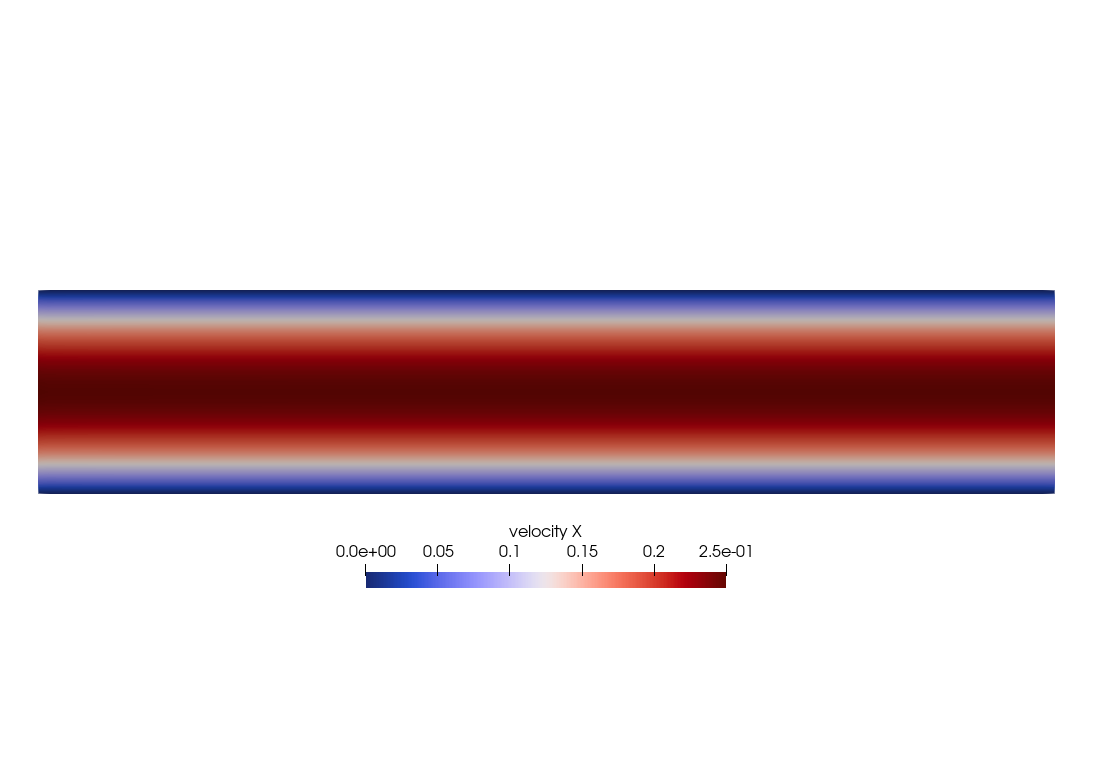
\includegraphics[width=5cm]{python_codes/fieldstone_72/results/mms2/u}
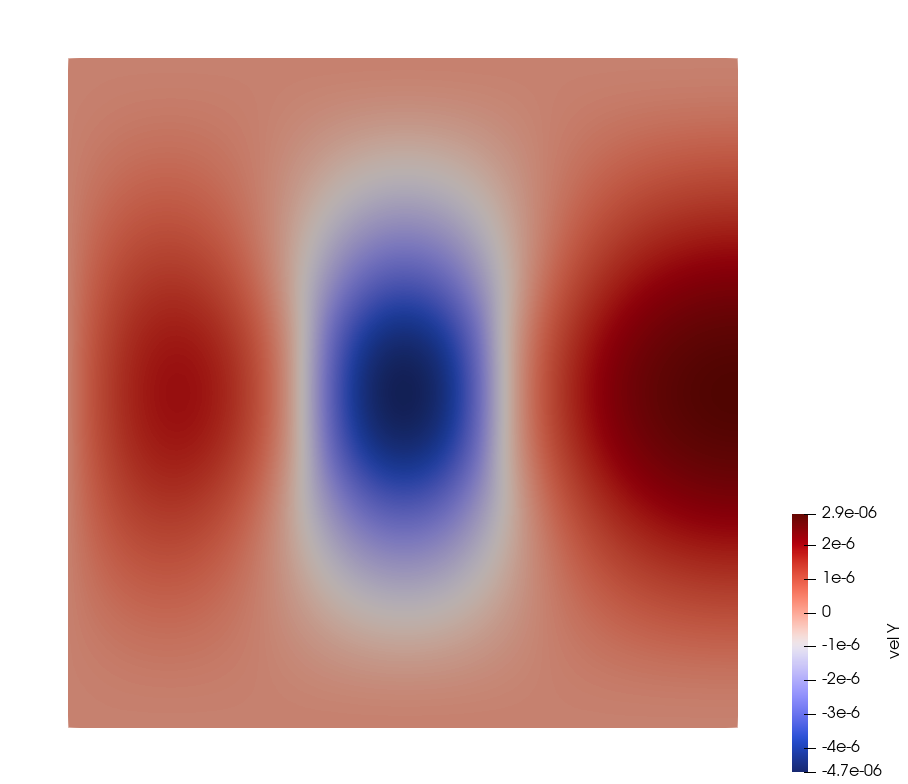
\includegraphics[width=5cm]{python_codes/fieldstone_72/results/mms2/v}
\includegraphics[width=5cm]{python_codes/fieldstone_72/results/mms2/vel}\\
{\captionfont Velocity field as obtained on $32\times 32$ grid. Left: $x-$component,
middle: $y-$component, right: velocity vector magnitude.}
\end{center}

\begin{center}
\includegraphics[width=7cm]{python_codes/fieldstone_72/results/mms2/error_v1}
\includegraphics[width=7cm]{python_codes/fieldstone_72/results/mms2/error_v2}\\
{\captionfont Velocity error for bubble function 1 (left) and bubble function 2 (right). 
$b_2$ maximum error is about half of $b_1$ error.}
\end{center}

\begin{center}
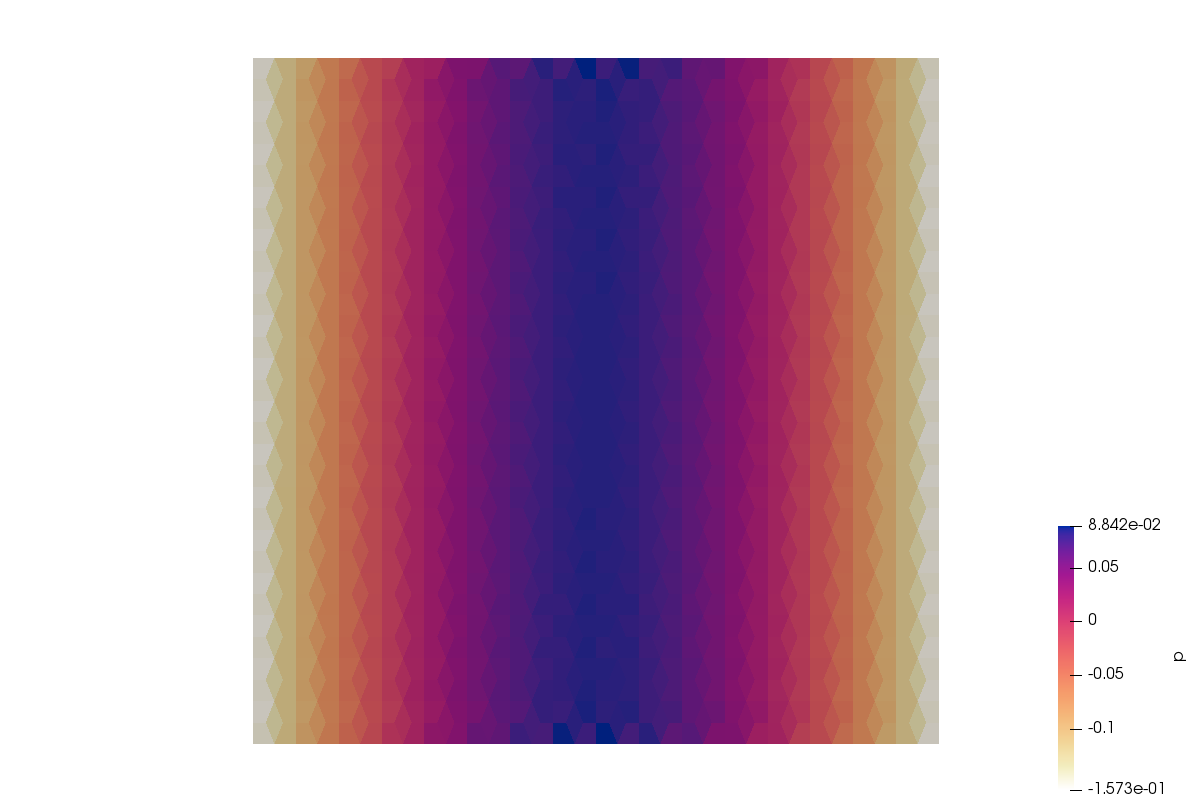
\includegraphics[width=7cm]{python_codes/fieldstone_72/results/mms2/p1}
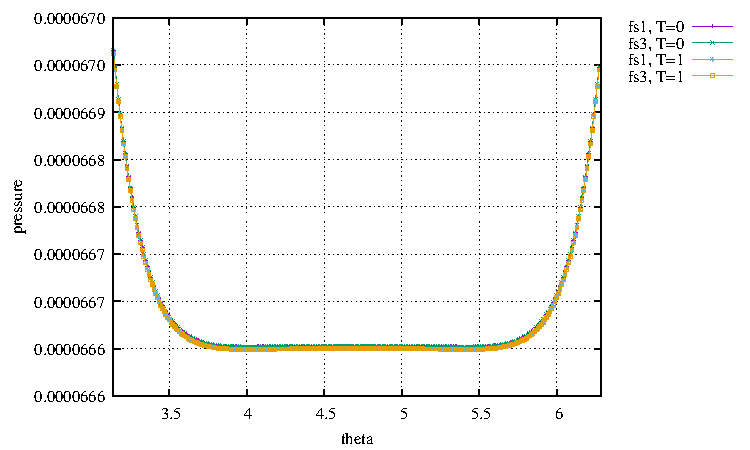
\includegraphics[width=7cm]{python_codes/fieldstone_72/results/mms2/p2}\\
{\captionfont Pressure field obtained with bubble function 1 (left) and bubble function 2 (right).
Scale has been voluntarily set to analytical values scale for both.}
\end{center}

\begin{center}
\includegraphics[width=7cm]{python_codes/fieldstone_72/results/mms2/error_p1}
\includegraphics[width=7cm]{python_codes/fieldstone_72/results/mms2/error_p2}\\
{\captionfont Pressure error field obtained with bubble function 1 (left) and bubble function 2 (right). Notice the 
different error magnitudes between both!}
\end{center}

The conclusions are identical to those obtained with the first manufactured solution. 
The second bubble function (here with $\beta=1/4$) performs better. While velocity error
convergence rates are quadratic for both bubbles, the pressure error is substantially lower
for bubble 2 (although its rate is slightly lower than bubble 1 -- both are still 
superconvergent). This is illustrated above where we see that the pressure field obtained 
with bubble 1 showcases strong ripples in the upper right corner.     



%_____________________________________
\section*{The SolCx benchmark}

Because of the viscosity jump at $x=L_x/2$, it has been widely reported that 
error convergence rates depend on wheter the number of element in the $x-$direction 
is even or odd.

\begin{center}
\includegraphics[width=5cm]{python_codes/fieldstone_72/results/solcx/errors_v_even}
\includegraphics[width=5cm]{python_codes/fieldstone_72/results/solcx/errors_p_even}
\includegraphics[width=5cm]{python_codes/fieldstone_72/results/solcx/vrms_even}\\
\includegraphics[width=5cm]{python_codes/fieldstone_72/results/solcx/errors_v_odd}
\includegraphics[width=5cm]{python_codes/fieldstone_72/results/solcx/errors_p_odd}
\includegraphics[width=5cm]{python_codes/fieldstone_72/results/solcx/vrms_odd}
\end{center}

Velocity error convergence rates are 2 for even numbers of elements and 1 for odd numbers, 
such as for the Q1Q1 stab. 
Pressure error convergence rate seems to be 0.5 for odd numbers of elements and
0.65 for even numbers ... 

\begin{center}
\includegraphics[width=5cm]{python_codes/fieldstone_72/results/solcx/vel}
\includegraphics[width=5cm]{python_codes/fieldstone_72/results/solcx/p}
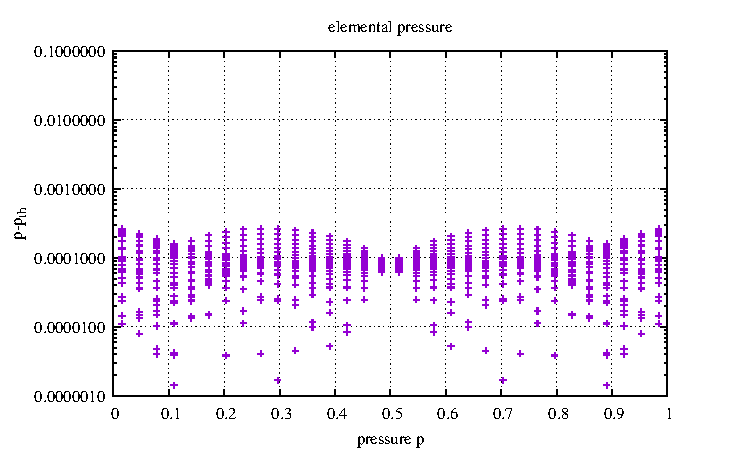
\includegraphics[width=5cm]{python_codes/fieldstone_72/results/solcx/p_error}
\end{center}

We see that the pressure showcases an strong error (even at high resolution)
along the interface. 


%_____________________________________
\section*{The SolKz benchmark}

\begin{center}
\includegraphics[width=5cm]{python_codes/fieldstone_72/results/solkz/errors_v}
\includegraphics[width=5cm]{python_codes/fieldstone_72/results/solkz/errors_p}
\includegraphics[width=5cm]{python_codes/fieldstone_72/results/solkz/vrms}
\end{center}

We find that velocity and pressure errors converge quadratically, with 
once again $b_2$ better than $b_1$.


%_____________________________________
\section*{The SolVi benchmark}


\begin{center}
\includegraphics[width=7cm]{python_codes/fieldstone_72/results/solvi/vel}
\includegraphics[width=7cm]{python_codes/fieldstone_72/results/solvi/p}\\
{\captionfont Resolution $128\times128$ - bubble 1 }
\end{center}


\begin{center}
\includegraphics[width=5cm]{python_codes/fieldstone_72/results/solvi/errors_v}
\includegraphics[width=5cm]{python_codes/fieldstone_72/results/solvi/errors_p}
\includegraphics[width=5cm]{python_codes/fieldstone_72/results/solvi/vrms}
\end{center}



%_____________________________________
\section*{The Stokes Sphere}

This experiment is the benchmark of Section~\ref{MMM-ss:stokes_sphere2D}. 
The density is assigned directly to the 
quadrature point by means of a function. Inside the disc of radius 0.123456789 centered in the domain 
the density is set to 1.01 while it is set to 1 outside 
(viscosities are respectively 1000 and 1). The gravity is $|g_y|=1$ and 
free-slip boundary conditions are implemented on all sides. 

On the following figures the min/max of the pressure in the domain and the vrms 
are shown for both bubble functions. We see that at low resolution the reported 
values show some variations but with increasing resolution the quantities converge to a single value:

\begin{center}
\includegraphics[width=7cm]{python_codes/fieldstone_72/results/sphere/pstats}
\includegraphics[width=7cm]{python_codes/fieldstone_72/results/sphere/vrms}
\end{center}

\begin{center}
\includegraphics[width=7cm]{python_codes/fieldstone_72/results/sphere/vel_b1}
\includegraphics[width=7cm]{python_codes/fieldstone_72/results/sphere/vel_b2}\\
\includegraphics[width=7cm]{python_codes/fieldstone_72/results/sphere/p_b1}
\includegraphics[width=7cm]{python_codes/fieldstone_72/results/sphere/p_b2}\\
{\captionfont Left is b1, Right is b2.}
\end{center}

It looks like $b_2$ yields more anomalous pressure modes inside the sphere, 
which is corroborated by the following figures which show the pressure 
at $x=L_x/2$ in both cases. However we also see that at high resolution both 
bubbles yield nearly identical pressure profiles and that the ripples have vanished. 

\begin{center}
\includegraphics[width=5cm]{python_codes/fieldstone_72/results/sphere/pline_b1_closed}
\includegraphics[width=5cm]{python_codes/fieldstone_72/results/sphere/pline_b2_closed}
\includegraphics[width=5cm]{python_codes/fieldstone_72/results/sphere/pline_b12_closed}\\
{\captionfont pressure profile for b1 (left) and b2 (middle) for different resolutions.}
\end{center}

One can also prescribe an open boundary condition at the top:

\begin{center}
\includegraphics[width=7cm]{python_codes/fieldstone_72/results/sphere/open/vel}
\includegraphics[width=7cm]{python_codes/fieldstone_72/results/sphere/open/p}
\end{center}


\begin{center}
\includegraphics[width=5cm]{python_codes/fieldstone_72/results/sphere/pline_b1_open}
\includegraphics[width=5cm]{python_codes/fieldstone_72/results/sphere/pline_b2_open}
\includegraphics[width=5cm]{python_codes/fieldstone_72/results/sphere/pline_b12_open}\\
{\captionfont pressure profile for b1 (left) and b2 (middle) for different resolutions.}
\end{center}





%_____________________________________
\section*{Rayleigh-Taylor instability}

This benchmark is carried out in Appendix D of Thieulot (2011) \cite{thie11}.
It consists of a two-layer system driven by gravity.
The mesh is modified so as to align with the sinusoidal perturbation.
Resolution and $\eta_2$ are varied on the following figures:

\begin{center}
\includegraphics[width=7cm]{python_codes/fieldstone_72/results/RT/area}
\includegraphics[width=7cm]{python_codes/fieldstone_72/results/RT/eta}\\
\includegraphics[width=7cm]{python_codes/fieldstone_72/results/RT/rho}
\includegraphics[width=7cm]{python_codes/fieldstone_72/results/RT/vel}
\end{center}


\begin{center}
\includegraphics[width=7cm]{python_codes/fieldstone_72/results/RT/vy_b1}
\includegraphics[width=7cm]{python_codes/fieldstone_72/results/RT/vy_b2}
\end{center}

Bubble 2 does better than bubble 1. Also, $\beta$ does not seem to play a role.

%_____________________________________
\section*{Sinking block}
This is the very same experiment as in Stone 53. It consists of a negatively buoyant 
square object falling in a fluid in a square domain. 
This particular experiment proved to be the 'downfall' of the $Q_1\times Q_1-stab$ element
since the stabilisation term is akin to a pressure diffusion and therefore
acts on the lithostatic pressure and also tends to smooth the effect of small 
density variations (Thieulot \& Bangerth, in prep.). 

Unless specified otherwise bubble 2 has $\beta=0.25$ by default.

%............................
\subsection*{Full density} 
Results indicate that the element performs adequately, especially the 
pressure field which looks smooth.  

\begin{center}
\includegraphics[width=7cm]{python_codes/fieldstone_72/results/block/full/density}
\includegraphics[width=7cm]{python_codes/fieldstone_72/results/block/full/viscosity}\\
\includegraphics[width=7cm]{python_codes/fieldstone_72/results/block/full/vel}
\includegraphics[width=7cm]{python_codes/fieldstone_72/results/block/full/p}\\
{\captionfont $64\times 64$. Viscosity ratio is 10, $\delta \rho=8$, bubble 1.}
\end{center}

We see that the element is capable of reprensenting a linear pressure profile
(the overpressure signal due to the block is negligible compared to the 
hydrostatic pressure).

\begin{center}
\includegraphics[width=10cm]{python_codes/fieldstone_72/results/block/full/plines}\\
{\captionfont Pressure profile measured at $x=L_x/2$ for various resolutions. Same parameters
as previous figure.}
\end{center}

As before we produce the characteristic figures of the velocity and pressure in the middle of the 
block as a function of the viscosity ratio and the density difference. The results obtained 
with the quadrilateral MINI element agree nicely with those obtained with the $Q_2\times Q_1$ element:
 
\begin{center}
\includegraphics[width=7cm]{python_codes/fieldstone_72/results/block/full/results_v}
\includegraphics[width=7cm]{python_codes/fieldstone_72/results/block/full/results_p}
\end{center}


\underline{Influence of $\beta$ parameter for bubble 2:} I set $\delta\rho=8$, resolution 64x64, $\eta^\star=10$,
and record the pressure profile 

\begin{center}
\includegraphics[width=10cm]{python_codes/fieldstone_72/results/block/full/betastudy/plines}
\end{center}

We can conclude that the bubble type and the value of $\beta$ do not seem to significantly affect 
the pressure profile in this case.

%............................
\subsection*{Reduced density} 
This is the same experiment as above but $\rho_1$ has been removed from the density
everywhere in the domain, so that the surrounding material has zero density 
and the block has a density $\delta \rho$.
The velocity and pressure field are then:

\begin{center}
\includegraphics[width=7cm]{python_codes/fieldstone_72/results/block/reduced/vel}
\includegraphics[width=7cm]{python_codes/fieldstone_72/results/block/reduced/p}\\
{\captionfont $64\times 64$. Viscosity ratio is 10, $\delta \rho=8$. bubble 1}
\end{center}

We then turn to the pressure along the vertical line $x=L_x/2$ as obtained with 
both bubble functions and find that both yield visually similar profiles:

\begin{center}
\includegraphics[width=7cm]{python_codes/fieldstone_72/results/block/reduced/plines_b1}
\includegraphics[width=7cm]{python_codes/fieldstone_72/results/block/reduced/plines_b2}\\
{\captionfont Pressure profile measured at $x=L_x/2$ for various resolutions and for both bubble functions.
Left is bubble 1, right is bubble 2.}
\end{center}

I hereafter plot the pressure profiles for both bubble functions at the highest resolution, i.e. $96\times 96$.
We see that differences are somewhat minimal, although bubble 2 yields a pressure above the block which 
showcases worrying oscillations. Also the results are remarquably similar to those obtained with the Taylor-Hood
$Q_2\times Q_1$ element:

\begin{center}
\includegraphics[width=7cm]{python_codes/fieldstone_72/results/block/reduced/plines_b12}
\includegraphics[width=7cm]{python_codes/fieldstone_72/results/block/reduced/plines_b12_zoom}
\end{center}

Finally the velocity and pressure inside the block unsurprisingly match nicely with those obtained with the Taylor-Hood
$Q_2\times Q_1$ element:

\begin{center}
\includegraphics[width=7cm]{python_codes/fieldstone_72/results/block/reduced/results_v}
\includegraphics[width=7cm]{python_codes/fieldstone_72/results/block/reduced/results_p}
\end{center}


\underline{Influence of $\beta$ parameter for bubble 2:} I set $\delta\rho=8$, resolution 64x64, $\eta^\star=10$,
and record the pressure profile 

\begin{center}
\includegraphics[width=7cm]{python_codes/fieldstone_72/results/block/reduced/betastudy/plines}
\includegraphics[width=7cm]{python_codes/fieldstone_72/results/block/reduced/betastudy/plines_zoom}
\end{center}

It is here very obvious that low values of $\beta$ yield problematic pressure oscillations. 
It looks like $\beta \geq 0.25$ actually yield near identical results to those obtained with bubble 1,
but $\beta=1$ or $\beta=2$ also yields unwanted oscillations.

%_____________________________________
\section*{Free surface benchmark}

The setup originates in Crameri et al (2012) \cite{crsg12}. It consists of 
a cosine-shaped layer of homogeneous lithosphere overlaying a homogeneous layer of mantle.
The domain is 2800x700 km. The amplitude of the surface perturbation is 7km. 
Free slip boundary conditions are prescribed on the sides and no-slip at the bottom. 
The lithosphere is characterised by $\eta=10^{23}$Pa.s and the mantle by $\eta=10^{21}$Pa.s, 
while both have a density of 3330kg/m3.

\begin{center}
\includegraphics[width=13cm]{python_codes/fieldstone_72/results/crsg12/area}\\
{\captionfont Setup of the mesh. Area of the elements.}
\end{center}

I do not wish to implement a mesh evolution algorithm nor timestepping so
I only report the velocity field at $t=0$:

\begin{center}
\includegraphics[width=7cm]{python_codes/fieldstone_72/results/crsg12/u}
\includegraphics[width=7cm]{python_codes/fieldstone_72/results/crsg12/v}\\
\includegraphics[width=7cm]{python_codes/fieldstone_72/results/crsg12/vel}
\includegraphics[width=7cm]{python_codes/fieldstone_72/results/crsg12/p}
\end{center}

It is clear that the velocity is (visually) what we expect. The presence of the free surface 
does not seem to introduce any kind of abnormal behaviour. 


\newpage
%%%%%%%%%%%%%%%%%%%%%%%%%%%%%%%%%%%%%%%%%%%%%%%%%%%%%%%%%%%%%%%%%%%%%%%%%%%%%%%
\section*{NEW stuff}

all in {\tt /study} folder.

Following \textcite{lami17} (2017), we consider the case of a 4x4 element mesh (macro-element).
We prescribe u and v boundary conditions on all sides (8 nodes) so that
16 lines of the G matrix are zero. Since the original G matrix is (9+4)*2=26 dofs, 
there are only 26-8*2 lines left, i.e. a 9*10 matrix like the D one of the paper.

%-----------------------
\subsection*{bubble 0}

%\begin{center}
%\includegraphics[width=10cm]{python_codes/fieldstone_72/images/mat1}\\
%{\captionfont ${\bm G}$ matrix obtained with the $(1-x^2)(1-y^2)$ bubble}
%\end{center}

The matrix shown in the paper is
\[
D=
\left(
\begin{array}{cccccccccc}
\frac29 & \frac29 & 0 & 0 & 0 & 0 & 0 & 0 & \frac{1}{12} & \frac{1}{12} \\ \\
-\frac29 & \frac29 & \frac29 & \frac29 & 0 & 0 & 0 & 0 & 0 & \frac13 \\ \\
0 & 0 & -\frac29 & \frac29 & 0 & 0 & 0 & 0 & -\frac{1}{12} & \frac{1}{12} \\ \\
\frac29 & -\frac29 & 0 & 0 & 0 & 0 & \frac29 & \frac29 & \frac13  & 0 \\ \\ 
-\frac29 & -\frac29 & \frac29 & -\frac29 & \frac29 & \frac29 & -\frac29 & \frac29  &0 &0\\ \\
0 & 0 & -\frac29 & -\frac29 & -\frac29 & \frac29 & 0 & 0 & -\frac13 & 0 \\ \\
0 & 0 & 0 & 0 & 0 & 0 & \frac29 & -\frac29 & \frac{1}{12} & -\frac{1}{12} \\ \\
0 & 0 & 0 & 0 & \frac29 & -\frac29 & -\frac29 & -\frac29 & 0 & -\frac13 \\ \\ 
0 & 0 & 0 & 0 & -\frac29 & -\frac29 & 0 & 0 & -\frac{1}{12} & -\frac{1}{12}
\end{array}
\right)
\]
which we can write: 
\[
D=
\frac19
\left(
\begin{array}{cccccccccc}
2 & 2 & 0 & 0 & 0 & 0 & 0 & 0 & \frac{3}{4} & \frac{3}{4} \\ \\
-2 & 2 & 2 & 2 & 0 & 0 & 0 & 0 & 0 & 3 \\ \\
0 & 0 & -2 & 2 & 0 & 0 & 0 & 0 & -\frac{3}{4} & \frac{3}{4} \\ \\
2 & -2 & 0 & 0 & 0 & 0 & 2 & 2 & 3  & 0 \\ \\ 
-2 & -2 & 2 & -2 & 2 & 2 & -2 & 2  &0 &0\\ \\
0 & 0 & -2 & -2 & -2 & 2 & 0 & 0 & -3 & 0 \\ \\
0 & 0 & 0 & 0 & 0 & 0 & 2 & -2 & \frac{3}{4} & -\frac{3}{4} \\ \\
0 & 0 & 0 & 0 & 2 & -2 & -2 & -2 & 0 & -3 \\ \\ 
0 & 0 & 0 & 0 & -2 & -2 & 0 & 0 & -\frac{3}{4} & -\frac{3}{4}
\end{array}
\right)
\]


Here is what I obtain (matrix multiplied by 9). Structure is good.
First 8 columns are perfect BUT last two columns are off, and not just 
by a single constant...rank is found to be 7 as in the paper.

\begin{verbatim}
[[ 2.    2.   -0.   -0.   -0.   -0.   -0.   -0.    0.25  0.25]
 [-2.    2.    2.    2.   -0.   -0.   -0.   -0.   -0.    2.  ]
 [-0.   -0.   -2.    2.   -0.   -0.   -0.   -0.   -0.25  0.25]
 [ 2.   -2.   -0.   -0.   -0.   -0.    2.    2.    2.   -0.  ]
 [-2.   -2.    2.   -2.    2.    2.   -2.    2.   -0.   -0.  ]
 [-0.   -0.   -2.   -2.   -2.    2.   -0.   -0.   -2.   -0.  ]
 [-0.   -0.   -0.   -0.   -0.   -0.    2.   -2.    0.25 -0.25]
 [-0.   -0.   -0.   -0.    2.   -2.   -2.   -2.   -0.   -2.  ]
 [-0.   -0.   -0.   -0.   -2.   -2.   -0.   -0.   -0.25 -0.25]]
\end{verbatim}

Let us investigate further and go back to the paper:
\begin{center}
\includegraphics[width=13cm]{python_codes/fieldstone_72/images/mat4}\\
\end{center}

In my notations:
\[
\left[
\iint \partial_x b_1 \bN_j^p dV,
\iint \partial_y b_1 \bN_j^p dV,
\iint \partial_x b_2 \bN_j^p dV,
\iint \partial_y b_2 \bN_j^p dV, ...
\iint \partial_x b_5 \bN_j^p dV,
\iint \partial_y b_5 \bN_j^p dV
\right]
\]
where the subscript of the bubble refers to the element and the integrals over the domain. 

Let us look at $j=1$ (i.e. first line of the matrix). Since function $N_1^p$ has compact support 
over element 1 only, we obtain
\begin{align}
\iint_{domain} \partial_x b_1 \bN_1^p dV
&= \iint_{elt 1} \partial_x b_1 \bN_1^p dV \\
&= \frac14 \iint_{ref elt} 2\partial_r b_1 \bN_1^p drds \\
&= \frac14 2\int_{-1}^{+1} \int_{-1}^{+1}  \partial_r [(1-r^2)(1-s^2)] \bN_1^p    dr ds \\
&= \frac14 2\int_{-1}^{+1}   \int_{-1}^{+1}  -2r (1-s^2) \frac14(1-r)(1-s)   dr ds \\
&= \frac14 2\int_{-1}^{+1} -2r(1-r) dr \cdot  \int_{-1}^{+1}  (1-s^2) (1-s) ds \\
&= \frac14 2 \frac43  \frac43  \\
&= \frac29
\end{align}

Let us now focus on $j=1$ again but this time we use the 
velocity basis function at node 5 (in the middle of the domain --see fig above).
In element 1 this node is node 3 with basis function $\frac14(1+r)(1+s)$.
Same story as above, pressure basis function compact support on elt 1 only
\begin{align}
\iint_{domain} \partial_x N_5 \bN_1^p dV
&= \iint_{elt1} \partial_x N_5 \bN_1^p dV \\
&= \frac14 \iint_{ref} 2 \partial_r [\frac14(1+r)(1+s)] \frac14 (1-r)(1-s) dV \\
&= \frac14 \frac14 \frac14 2 \int_{-1}^{+1}   \int_{-1}^{+1} (1+s)  (1-r)(1-s) dV \\
&= \frac14 \frac14 \frac14 2 \int_{-1}^{+1} (1-r) dr \int_{-1}^{+1} (1-s^2) ds \\
&= \frac14 \frac14 \frac14 2 2 \frac43 \\
&= \frac{1}{12} 
\end{align}
Although it aligns with the values in the paper, I believe it is {\it wrong}. 
Indeed, the basis function for node 3 in element 1 is not $\frac14(1+r)(1+s)$
but $\frac14(1+r)(1+s)-\frac14 b(r,s)$ (see Section~\ref{MMM-eq:miniN12345}).
In this case, 
\begin{align}
\iint_{domain} \partial_x N_5 \bN_1^p dV
&= \iint_{elt1} \partial_x N_5 \bN_1^p dV \\
&= \frac14 \iint_{ref} 2 \partial_r \left[\frac14(1+r)(1+s) -\frac14b(r,s) \right] \frac14 (1-r)(1-s) dr ds \\
&=  \frac14 \frac14 \frac14 2 \int_{-1}^{+1} \int_{-1}^{+1} (1+s)  (1-r)(1-s) dr ds
- \frac14 \frac14 \frac14 2 \int_{-1}^{+1} \int_{-1}^{+1} \partial_r b(r,s) (1-r)(1-s) dr ds
\end{align}
and in the case of bubble 0:
\begin{align}
&\frac14 \frac14 \frac14 2 \int_{-1}^{+1} \int_{-1}^{+1} \partial_r b(r,s) (1-r)(1-s) dV \nonumber\\ 
&= \frac14 \frac14 \frac14 2 \int_{-1}^{+1} \int_{-1}^{+1} \partial_r [(1-r^2)(1-s^2)] (1-r)(1-s) dr ds \nonumber\\ 
&= \frac14 \frac14 \frac14 2 \int_{-1}^{+1} \int_{-1}^{+1} -2r(1-s^2) (1-r)(1-s) dr ds \nonumber\\ 
&= \frac14 \frac14 \frac14 2 \int_{-1}^{+1}  -2r(1-r)  dr \int_{-1}^{+1} (1-s^2) (1-s) ds \nonumber\\ 
&= \frac14 \frac14 \frac14 2 \frac43 \frac43 \nonumber\\
&= \frac{1}{18}
\end{align}
In the end, 
\[
\iint_{domain} \partial_x N_5 \bN_1^p dV
= \frac{1}{12} - \frac{1}{18}
= \frac{3}{36} - \frac{2}{36} 
= \frac{1}{36}
= \frac{1}{9} \frac{1}{4}
\]
and we recover the value $1/4$. 

Let us now turn to the second line ($j=2$). The pressure basis function has compact support
over elements 1 and 2. In elt 1 it is $\frac14(1+r)(1-s)$ and in elt2 it is $\frac14(1-r)(1-s)$.
The velocity basis fct at node 5 is $\frac14(1+r)(1+s)-\frac14 b$ in element 1 and 
$\frac14(1-r)(1+s) -\frac14 b$ in elt 2. In the end:

\begin{align}
&\iint_{domain} \partial_x N_5 \bN_2^p dV \nonumber\\
&= \iint_{elt1} \partial_x N_5 \bN_2^p dV + \iint_{elt2} \partial_x N_5 \bN_2^p dV \nonumber\\
&= 
\frac14 \iint_{elt1} 2\partial_r [\frac14(1+r)(1+s)-\frac14 b] \frac14(1+r)(1-s) drds +
\frac14 \iint_{elt2} 2\partial_r [\frac14(1-r)(1+s)-\frac14 b] \frac14(1-r)(1-s) drds \nonumber\\
&=
\frac14\frac14\frac14 2 
\left[ 
\iint_{elt1} \partial_r [(1+r)(1+s)-b] (1+r)(1-s) drds +
\iint_{elt2} \partial_r [(1-r)(1+s)-b] (1-r)(1-s) drds 
\right] \nonumber\\
&=
\frac14\frac14\frac14 2 
\left[ 
\int_{-1}^{+1} \int_{-1}^{+1}  [ (1+s)-\partial_r b] (1+r)(1-s) drds +
\int_{-1}^{+1} \int_{-1}^{+1}  [-(1+s)-\partial_r b] (1-r)(1-s) drds 
\right] \nonumber\\
&= 
\frac14\frac14\frac14 2 
\left[ 
\int_{-1}^{+1} \int_{-1}^{+1}  [ (1+s) +2r(1-s^2)] (1+r)(1-s) drds +
\int_{-1}^{+1} \int_{-1}^{+1}  [-(1+s) +2r(1-s^2)] (1-r)(1-s) drds
\right] \nonumber\\ 
&= 4.4444... -4.44444 \nonumber\\ 
&= 0
\end{align}
(thank you Wolfram Alpha)


Note that in the case of a pressure field, its gradient should be zero. 
This means that the sum of all numbers on a given column of this matrix 
should be zero, which is the case for both my and his matrix.

Interestingly, we can compute the null space of the $D^T$ matrix (.i.e $\G$).
We obtain
\begin{verbatim}
[[-0.11773066 -0.43143886]
 [ 0.48236331 -0.13162688]
 [-0.11773066 -0.43143886]
 [ 0.48236331 -0.13162688]
 [-0.11773066 -0.43143886]
 [ 0.48236331 -0.13162688]
 [-0.11773066 -0.43143886]
 [ 0.48236331 -0.13162688]
 [-0.11773066 -0.43143886]]
\end{verbatim}
It is of size two, which is problematic since the only vector in the 
null space should be the vector of constant pressures.

\newpage
%-----------------------
\subsection*{bubble 1}

\begin{center}
\includegraphics[width=10cm]{python_codes/fieldstone_72/images/mat2}\\
{\captionfont ${\bm G}$ matrix obtained with the $(1-x^2)(1-y^2)(1-x)(1-y)$ bubble}
\end{center}

after multiplying by 27/4
\begin{verbatim}
[[ 2.      2.     -0.     -0.     -0.     -0.     -0.     -0.      0.0625  0.0625]
 [-2.      1.      2.      2.     -0.     -0.     -0.     -0.     -0.      1.5   ]
 [-0.     -0.     -2.      1.     -0.     -0.     -0.     -0.     -0.0625  0.3125]
 [ 1.     -2.     -0.     -0.     -0.     -0.      2.      2.      1.5    -0.    ]
 [-1.     -1.      1.     -2.      2.      2.     -2.      1.     -0.     -0.    ]
 [-0.     -0.     -1.     -1.     -2.      1.     -0.     -0.     -1.5    -0.    ]
 [-0.     -0.     -0.     -0.     -0.     -0.      1.     -2.      0.3125 -0.0625]
 [-0.     -0.     -0.     -0.      1.     -2.     -1.     -1.     -0.     -1.5   ]
 [-0.     -0.     -0.     -0.     -1.     -1.     -0.     -0.     -0.3125 -0.3125]]
\end{verbatim}

For reasons being made evident in the bubble 0 case, I cannot obtain the same 
matrix as he does in the paper. I should still at some point investigate in detail why
and do a few calculations to be sure I understand how he obtained his coeffs. 

rank is 8

We can compute the null space of the $D^T$ matrix (.i.e $\G$).
We obtain
\begin{verbatim}
[[-0.33333333]
 [-0.33333333]
 [-0.33333333]
 [-0.33333333]
 [-0.33333333]
 [-0.33333333]
 [-0.33333333]
 [-0.33333333]
 [-0.33333333]]
\end{verbatim}
It is of size one and is the vector of constant pressures, as expected.


%-----------------------
\subsection*{bubble 2}

\begin{center}
\includegraphics[width=10cm]{python_codes/fieldstone_72/images/mat3}\\
{\captionfont ${\bm G}$ matrix obtained with the $(1-x^2)(1-y^2)(1+x/4+y/4)$ bubble}
\end{center}

after multiplying by 18*3
\begin{verbatim}
[[ 11.    11.    -0.    -0.    -0.    -0.    -0.    -0.     1.75   1.75]
 [-11.    13.    11.    11.    -0.    -0.    -0.    -0.    -0.    12.  ]
 [ -0.    -0.   -11.    13.    -0.    -0.    -0.    -0.    -1.75   1.25]
 [ 13.   -11.    -0.    -0.    -0.    -0.    11.    11.    12.    -0.  ]
 [-13.   -13.    13.   -11.    11.    11.   -11.    13.    -0.    -0.  ]
 [ -0.    -0.   -13.   -13.   -11.    13.    -0.    -0.   -12.    -0.  ]
 [ -0.    -0.    -0.    -0.    -0.    -0.    13.   -11.     1.25  -1.75]
 [ -0.    -0.    -0.    -0.    13.   -11.   -13.   -13.    -0.   -12.  ]
 [ -0.    -0.    -0.    -0.   -13.   -13.    -0.    -0.    -1.25  -1.25]]
\end{verbatim}

For reasons being made evident in the bubble 0 case, I cannot obtain the same 
matrix as he does in the paper. 

rank is 8

We can compute the null space of the $D^T$ matrix (.i.e $\G$).
We obtain
\begin{verbatim}
[[0.33333333]
 [0.33333333]
 [0.33333333]
 [0.33333333]
 [0.33333333]
 [0.33333333]
 [0.33333333]
 [0.33333333]
 [0.33333333]]
\end{verbatim}
It is of size one and is the vector of constant pressures, as expected.




\newpage
%---------------------------------
\subsection*{let us reflect....}

Bubbles are postulated to be of the form
\[
b(r,s) = (1-r^2)(1-s^2) (1 + ar + bs + crs  )
\]
Bubble 0 corresponds to $a=b=c=0$. 
Bubble 1 corresponds to $a=-1$, $b=-1$, $c=1$
Bubble 2 corresponds to $a=\frac14$, $b=\frac14$, $c=0$

Bubble 0 does not yield a stable formulation, while bubbles 1\&2 do. 
The question is then: how many $a,b,c$ combinations yield stable formulations?

In order to answer this, I need to compute the $D$ matrix of the paper
as a function of $a,b,c$. Then I need to establish its rank as a function of $a,b,c$...

For example, I can run {\tt script\_run\_beta} for $\beta\in [0..100]$. 
I seems that any nonzero value of $\beta$ yields a rank equal to 8.
\begin{verbatim}
beta= 0.0 rank= 7
beta= 1e-06 rank= 8
beta= 2e-06 rank= 8
beta= 5e-06 rank= 8
beta= 1e-05 rank= 8
beta= 5e-05 rank= 8
beta= 0.0001 rank= 8
beta= 0.0005 rank= 8
beta= 0.001 rank= 8
beta= 0.005 rank= 8
beta= 0.01 rank= 8
beta= 0.02 rank= 8
beta= 0.05 rank= 8
beta= 0.1 rank= 8
beta= 0.25 rank= 8
beta= 0.5 rank= 8
beta= 1.0 rank= 8
beta= 2.0 rank= 8
beta= 5.0 rank= 8
beta= 10.0 rank= 8
beta= 100.0 rank= 8
\end{verbatim}


